\documentclass[a4paper, UKenglish]{article}
\usepackage[utf8]{inputenc}
\usepackage{babel}
\usepackage{amsmath}
\usepackage{graphicx}
\usepackage{mdframed}
\usepackage{listings}

\usepackage{color}
%\definecolor{deepblue}{rgb}{0,0,0.5}
%\definecolor{deepred}{rgb}{0.6,0,0}
%\definecolor{deepgreen}{rgb}{0,0.5,0}
\definecolor{mygrey}{gray}{0.9}
\definecolor{grey2}{gray}{0.95}

\newenvironment{print}{\begin{mdframed}[backgroundcolor=grey2,linecolor=grey2]\begin{lstlisting}}{\end{lstlisting}\end{mdframed}}

%opening
\title{Numerical Methods Exam Project: Bilinear Interpolation}
\author{Markus R. Mosbech}

\begin{document}

\maketitle

\begin{abstract}
\noindent I have made a program for two dimensional bilinear interpolation on rectilinear grids in two dimensions. I have made two different interpolation routines in order to determine which one is fastest.
\end{abstract}
\section{The Interpolator}
My interpolator consists of a single function. It takes an x-value and an y-value, both passed as doubles, to determine where to calculate the interpolated function. To interpolate, it also takes a pointer to a gsl\textunderscore{}matrix of tabulated function values and well as pointers to gsl\textunderscore{}vectors with x- and y-values at the tabulated points.
\begin{mdframed}[backgroundcolor=mygrey,linecolor=mygrey]
	\begin{lstlisting}[language=c]
double interp_bilin(double x, double y,
	 gsl_vector * X, gsl_vector * Y, gsl_matrix * F)
	\end{lstlisting}
\end{mdframed}
It returns the interpolated value at the given point as a double.

\section{Regular Grids}
The simplest task is to interpolate values between regularly spaced points. This is done for several example functions by the program main, found in the Regular\textunderscore{}grid-folder. Which functions and how many points are determined in main.c. Here are variables \textbf{Nx} and \textbf{Ny} determining the number of tabulated function points in the x- and y-directions, and \textbf{nx} and \textbf{ny} determining how many points to interpolate. The functions I interpolate as examples are the Rosenbrock function, the Himmelblau function, a 2d-Gaussian and a simple x+y-function. Heatmap plots of all these functions and the interpolated values can be found in the folder. The the x- and y-values of the tabulated points are shown in gridpoints.svg. An example is shown in figure \ref{fig:regular}.

\begin{figure}
	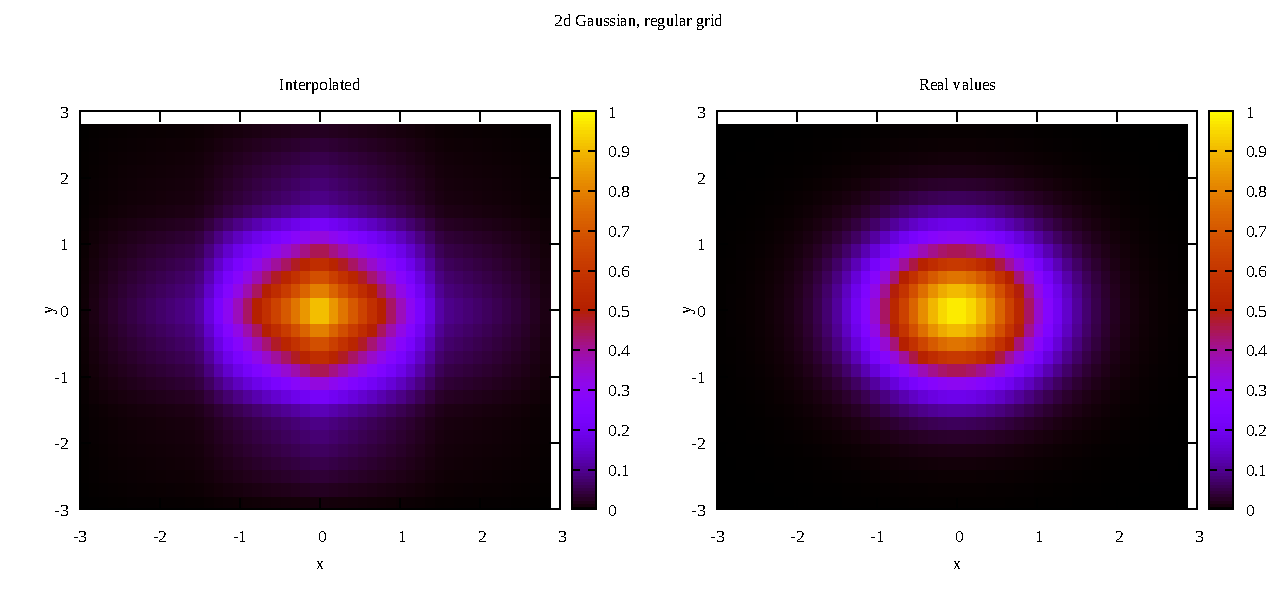
\includegraphics[width=\linewidth]{regular.pdf}
	\caption{Plot of 2d gaussian and interpolation on a regular grid.}
	\label{fig:regular}
\end{figure}

\section{Irregular Grids}
The interpolator works just as well for irregular grids. It is tested for the same functions, this is found in the folder Irregular\textunderscore{}grid. Here, x- and y-values of points were chosen at random between a given maximum and minimum value. Again, x- and y-values of the tabulated points are shown in gridpoints.svg. It is evident that the interpolation is more accurate in areas with higher density of tabulated points. This is of course to be expected. An example is shown in figure \ref{fig:irregular}.





\begin{figure}
	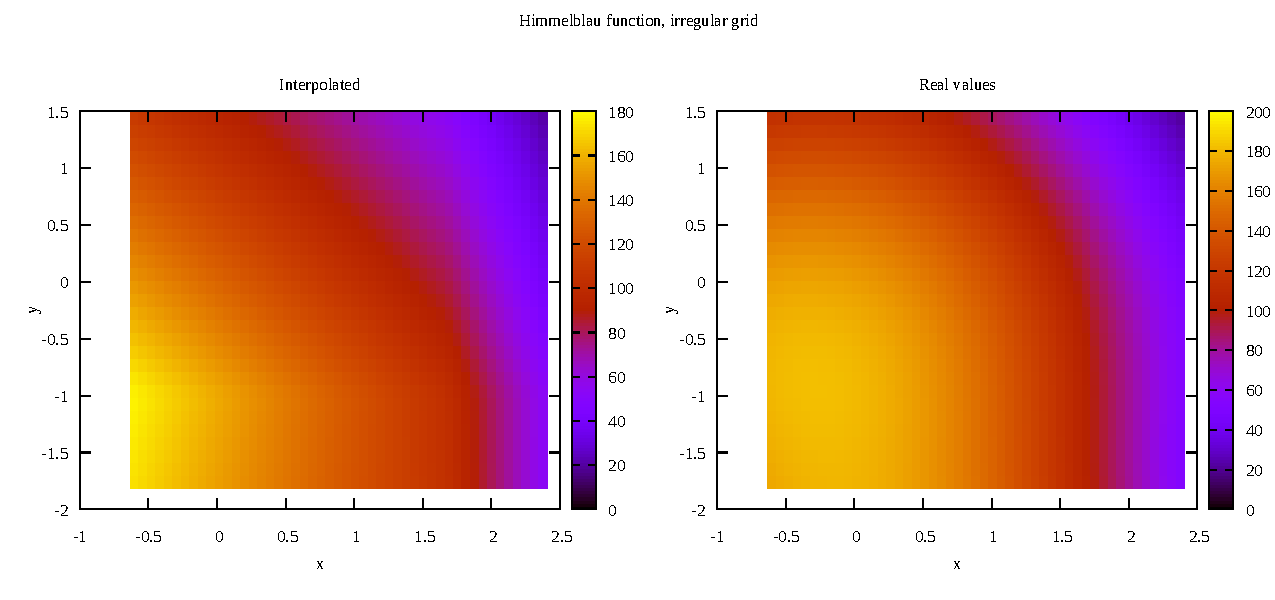
\includegraphics[width=\linewidth]{irregular.pdf}
	\caption{Plot of Himmelblau function and interpolation on an irregular grid.}
	\label{fig:irregular}
\end{figure}

\section{Comparison}
I came up with the idea of making an interpolator that calculates the function variables upon allocation and when calculating interpolated values just finds them in the allocated structure, similar to e.g. a one-dimensional cubic spline. There are thus 3 functions for this interpolator:

\hspace{-0.5cm}\begin{minipage}{\linewidth}
	\begin{mdframed}[backgroundcolor=mygrey,linecolor=mygrey]
		\begin{lstlisting}[language=c]
bilin * bilin_alloc(gsl_vector * X, gsl_vector *Y, 
			gsl_matrix * F);
double bilin2_interp(double x, double y, bilin * sys);
void bilin_free(bilin * sys);
		\end{lstlisting}
	\end{mdframed}
\end{minipage}
It uses the bilin structure, defined as
\begin{mdframed}[backgroundcolor=mygrey,linecolor=mygrey]
	\begin{lstlisting}[language=c]
typedef struct {
gsl_vector* X;
gsl_vector* Y;
gsl_matrix* a;
gsl_matrix* b;
gsl_matrix* c;
gsl_matrix* d;
} bilin;
	\end{lstlisting}
\end{mdframed}
I thought this might be more efficient for high numbers of interpolation calls, since the values of \textbf{a}, \textbf{b}, \textbf{c} and \textbf{d} would no have to be recalculated every time, merely drawn from a matrix. It turns out however, that the two interpolators are very equal in the time they take to calculate interpolated points, suggesting that most of the time is spent finding the right interval to use. This can be seen in figure \ref{fig:times}.
\begin{figure}
	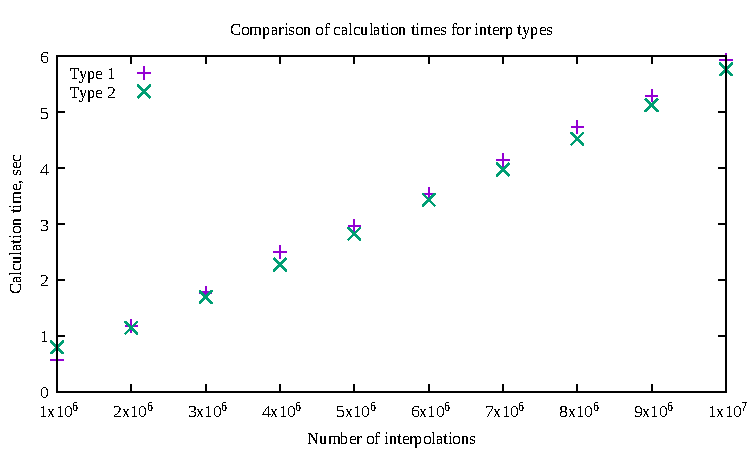
\includegraphics{times.pdf}
	\caption{Plot of calculation times for the two different interpolators as function of number of points calculated.}
	\label{fig:times}
\end{figure}

The test2test program was used to determine that the second type of interpolator does in fact work as intended. All this can be found in the Comparison folder.

\end{document}
